\documentclass[PWPL]{article}
\usepackage{PWPL}
\usepackage{tipa}
\usepackage{enumerate}
\usepackage{float}
\usepackage{graphicx}
\usepackage{multirow}
\usepackage{amsmath}
\usepackage{caption}
\usepackage{subfigure}
\title{The Social Perception of a Sound Change in York, Northern England}
\author{Daniel Lawrence}
\begin{document}
\maketitle
\abstract{A core claim of sociolinguistic theory is that language variation functions as a social-semiotic resource, providing an explanation for patterns of group-level convergence and divergence with regard to ongoing linguistic change. What is lacking from existing work is a framework for formulating testable hypotheses regarding the relationship between listeners’ social perceptions of innovations and their productive behavior with regard to those innovations. With a view to addressing this problem, this paper presents an account of the fronting and diphthongization of the tense back vowels /u/ and /o/ in York, Northern England. After presenting evidence of ongoing change in these vowels, the paper evaluates a recent account of the role of social indexicality in constraining the changes through a novel experimental paradigm. The findings contradict previous accounts of change in this community -- for example, despite its rapid and uniform incrementation and apparent lack of class-stratification in production, /u/-fronting emerges as a robust cue to socioeconomic status in perception. While the absence of fronted /o/ monophthongs in the speech of younger speakers has previously been interpreted as evidence of their stigmatization, there is no support for this in the perception data. Intriguingly, there is evidence of structured variability in listeners’ social-perceptual responses -- the social groups who lead the changes in production appear to be more sensitive to their social-indexical significance in perception.}

\section{Introduction}

\section{Data \& methods}

\subsection{Sampling}

Data are taken from a corpus of recordings collected from a convenience sample of 52 York residents born between 1935 and 2000. All participants were born and raised in York, and had at least one parent from York.Table 1 provides the basic demographic information of the sample, including participants' gender and year of birth (collected from a post-interview questionnaire), and their grouping according to a \textit{mobility index}. This index was one of three factors derived from informants' responses to the interview questions (see section x.x).

\vspace*{6pt}
\begin{table}[htbp]
\centering
\begin{tabular}{l|l|l|l|l}
Mobility index&\multicolumn{2}{l|}{Upper}&\multicolumn{2}{l}{Lower}\\
\hline
Gender& Female& Male & Female & Male\\
\hline
1935-1960 & 6&5&2&2\\
 1961-1980& 2 &4&4&0\\
1981-2000&  8&11&3&5\\

\end{tabular}
\caption{Characteristics of the speaker sample}
\end{table}
\vspace*{6pt}

\subsection{Social coding}

In addition to collecting each speaker's year of birth and gender, three social indices were created based on a set of questions asked during the sociolinguistic interview. Three underlying dimensions were derived from an exploratory factor analysis of these responses -- a general SES index, a local identity index, and a mobility index; for brevity, the specific details of this factor analysis will be left for a future version of this work. The general SES index groups together a measure of the speaker's level of education and employment status. The local identity index measures the degree to which each individual identifies as someone from York, and the extent to which they are invested in the local community. The mobility index groups together a set of characteristics related to geographical and social mobility, e.g. whether or not the speaker travels regularly within the UK; whether or not they have worked and studied in York for an extended period, and whether or not they plan to stay in York permanently.

\subsection{Production data}

The data include a) a 100-item wordlist, including 15 tokens of each vowel in a range of phonetic environments plus fillers; b) a map task (Anderson et al., 1991) using a selection of words from the word list and c) a sociolinguistic interview, including a range of questions relevant to the speakers' social background and identity with regard to York and the north of England. 

Vowels were segmented from the first to the last glottal pulse visible in the spectrogram, and measurements of F1, F2 and F3 were taken at 20 equidistant points along the vowel trajectory. The present analysis will focus on F2 trajectories, which provide a relatively reliable reflection of the degree of fronting and diphthongization for these vowels. Measurements were normalized using the centroid method of Watt \& Fabricius (2002), using the mean midpoint values of each speakers' \textipa{/A/} and \textipa{/i/} productions as reference values. The formant values provided in the present analyses are of the form $F^n/S (F^n)$, i.e. the ratio of the measured frequency in Hz to the centroid frequency of that formant for the speaker being analyzed.

\subsection{Perception tasks}

\subsubsection{Auditory stimuli}

The auditory stimuli consisted of resynthesized tokens of the following lexical items:

\begin{table}[!ht]
\centering
\label{my-label}
\begin{tabular}{lll}
Vowel& \multicolumn{2}{l}{Lexical items}            \\
\textipa{/u/}       & \textit{food}            & \textit{too}            \\
\textipa{/o/}     & \textit{toast}            & \textit{so}            
\end{tabular}
\end{table}


The words were read by a 24-year-old middle-class speaker from York as part of a larger word list, which included monosyllabic tokens representing the entire vowel inventory. The speaker was recorded in a soundproof recording booth using a Shure condenser microphone. The stimuli were resynthesized using a \textit{Praat} script based on Alku et al.'s (1999) \textit{IAIF} method. The complete set of \textipa{/o/} stimuli included tokens representing three steps of fronting of monophthongal variants and three steps of two types of fronting (targeting the vowel onset and offglide) across diphthongal tokens. These included a back diphthongal realization, two steps of fronting at the vowel onset, and two steps of fronting of the offglide. The \textsc{/u/} stimuli included examples of three levels of fronting, from a back realization to very fronted, as well as three identical tokens with lowered onsets, resulting in more diphthongal tokens.

Figures 3.1-3.3 give the IPA symbols which will be used to refer to the tokens in the analyses. 

\begin{table}[H]
\caption*{Figure 3.2: \textsc{goat} variants used in the experiment}
\centering
\footnotesize
\begin{tabular}{llllll}
&&&&&\\
                  &           & \textit{Fronting}          &             &                   &\\
                &  \multicolumn{3}{l}{$\xleftarrow{\hspace*{10cm}}$  }   &                              \\
\multirow{5}{*}{$\rotatebox[origin=c]{90}{$\underleftarrow{Diphthongization}$}$}                 &&&& &                \\
               & \LARGE{\textbf{\textipa{\o:}}}&\LARGE{\textbf{\textipa{8:}}}&\LARGE{\textbf{\textipa{o:}}}&&\\
 & Mid-front monophthong & Mid-central monophthong  & Mid-back monophthong  &         &          \\
        &\LARGE{\textbf{\textipa{eU}}}&\LARGE{\textbf{\textipa{9U}}}&\LARGE{\textbf{\textipa{oU}}}&&\\
                   & Mid-front diphthong  & Mid-central diphthong & Mid-back diphthong\\
                   &(fronted onset)&(centralized onset)&&&\\
                   &\LARGE{\textbf{\textipa{9y}}}&\LARGE{\textbf{\textipa{90}}}&&&\\
                   &Mid-front diphthong &Mid-central diphthong &&&\\
                   &(fronted offglide)&(centralized offglide)&&&\\
\end{tabular}
\end{table}
\begin{table}[H]
\caption*{Figure 3.3: \textsc{goose} variants used in the experiment}
\centering
\begin{tabular}{llllll}
&&&&&\\
                  &           & \textit{Fronting}          &             &                   &\\
            &  \multicolumn{3}{l}{$\xleftarrow{\hspace*{8cm}}$  }  &                              \\
                      
 &&&&\multirow{5}{*}{$\rotatebox[origin=c]{90}{$\overrightarrow{\hspace*{0.5cm}Raising\hspace*{0.5cm}}$}$}       &\\
        &\LARGE{\textbf{\textipa{Yu}}}&\LARGE{\textbf{\textipa{0u}}}&\LARGE{\textbf{\textipa{Uu}}}&&\\
                   & High-front  & High-central& High-back\\
               & \LARGE{\textbf{\textipa{eu}}}&\LARGE{\textbf{\textipa{9u}}}&\LARGE{\textbf{\textipa{7u}}}&&\\
       & High-front  & High-central& High-back\\
 & (lowered onset)  & (lowered onset)  &(lowered onset) \\
\end{tabular}
\end{table}

\subsubsection{Visual stimuli}

Visual stimuli consisted of eight images representing individuals of different ages (older vs younger), different occupations (working class vs middle class) and of different regional background (urban vs rural).  The social dimensions of older/younger, working-class/middle-class, and urban/rural were included based on the findings of a set of ethnographic interviews conducted prior to the main data collection phase, as well as the claims made by Haddican et al. (2013). Each stimulus image contained three components -- an image of a face (providing information about the character's age), an image of a place of work/study (providing information about the character's social status) and an image of an urban or rural location (providing information about the regional background of the character). The eight images represent all possible combinations of these three social dimensions, shown in Figure 3.7.

\subcapcentertrue
\begin{figure}[H]
\caption*{Figure 3.7: Visual stimuli}
\centering
\subfigure[Older, Middle-class, Rural]{
    
\includegraphics[scale=0.35]{M_O_MC_L_1.png}
    \label{fig:subfig1}
}
\subfigure[Younger, Middle-class, Rural]{
    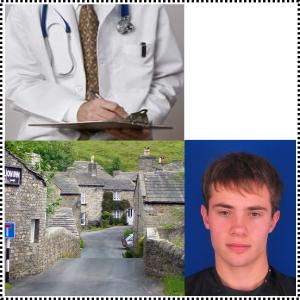
\includegraphics[scale=0.35]{M_Y_MC_L_1.png}
\label{fig:subfig2}
}
\subfigure[Older, Working-class, Rural]{
    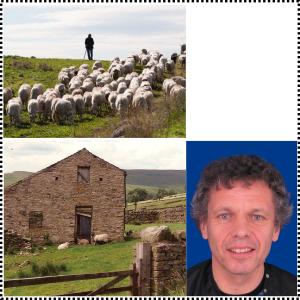
\includegraphics[scale=0.35]{M_O_WC_L_1.png}
    \label{fig:subfig3}
}
\subfigure[Younger, Working-class, Rural]{
    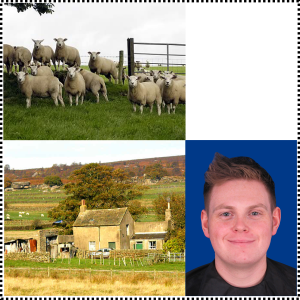
\includegraphics[scale=0.35]{M_Y_WC_L_1.png}
    \label{fig:subfig4}
}
\subfigure[Older, Middle-class, Urban]{
     
\includegraphics[scale=0.35]{M_O_MC_NL_1.png}
    \label{fig:subfig5}
}
\subfigure[Younger, Middle-class, Urban]{
      
\includegraphics[scale=0.35]{M_Y_MC_NL_1.png}
    \label{fig:subfig6}
}
\subfigure[Older, Working-class, Urban]{
      
\includegraphics[scale=0.35]{M_O_WC_NL_1.png}
    \label{fig:subfig7}
}
\subfigure[Younger, Working-class, Urban]{
         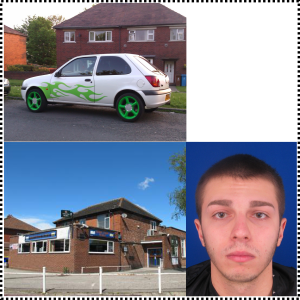
\includegraphics[scale=0.35]{M_Y_WC_NL_1.png}
    \label{fig:subfig8}
}
\end{figure}
The characters were designed to be feasible York personae, based on stereotypes discussed in the ethnographic interviews. Thus, the intersection of older, middle-class, and rural is represented by a doctor in a rural Yorkshire village (a), while the corresponding middle-class character is represented as a middle-aged businessman associated with a well-known insurance company (e). In all cases, the choice of component images reflects comments made by participants during the ethnographic interviews. The places used are those mentioned by the participants as being socially meaningful -- for example, the building in image (h) is Tang Hall Working Men's Club, a landmark in the Tang Hall area, which was repeatedly mentioned as being a rough, lower-class area. In contrast, the townhouses in image (e) are in The Mount, which was often contrasted with Tang Hall as being a more affluent area. The occupations chosen are those mentioned by participants, reflecting the stereotypes relevant to this social context. A key claim made by Haddican et. al. (2013) is that fronted monophthongal \textsc{goat} variants are associated with a working-class youth stereotype called a `chav'. In this experiment, the `chav' is treated as the intersection of the urban, young and working-class dimensions, represented by the character in image (h).

The non-facial images were taken from public domain collections, and the faces were selected from the Stirling ESRC facial database (http://pics.stir.ac.uk/ESRC/). The facial images were selected based on a pre-rating task completed by 20 students at the University of York. Since faces are potentially very rich sources of social information, two stimuli sets were created, by exchanging the pairs of faces within each age and social class combination (e.g. item (a) in the second stimuli set had the facial image from (e) and vice-versa). Distributing these face sets evenly across participants allowed any effect of the faces to be accounted for.

\subsubsection{Experimental task}

Participants were given the following instructions before starting the main experiment:\\\\
\textit{In the next part of the experiment, you will listen to the actor say a word and see two of the characters. Your task is to try and guess who the actor is pretending to be, by selecting one of the characters. Listen carefully to the way each word is pronounced, and choose the character who you think is the best match. To select the character, place your fingers on the `e' and `i' keys. These represent the two images which you will see on the screen. To select the right-hand box, press the `'i' key. To select the left-hand box, press the `e' key. Your responses will be timed, so please choose as quickly as possible. Sometimes you might feel that none of the speakers really match the sound you hear. If that's the case, just give your best guess.}\\

During the experiment, participants saw two images per trial and heard a speech token. The two images on each trial differed in terms of one of the three social dimensions, with the remaining two kept constant between each image pair. For example, participants would see older and younger rural, working class characters in a single trial, but an older working class and younger middle class character would never appear together. Altogether, this resulted in 12 image combinations which were presented with each of the 32 speech samples. Participants were given two breaks at one-third and two-thirds of the experiment, where they were encouraged to take a brief rest and re-start when ready.

The following section will outline the key findings from the production analysis, before using them to formulate and test predictions regarding the social perception data.

\section{The fronting of the tense back vowels in York, Northern England}
\subsection{The fronting and diphthongization of /u/ and /o/}
Figures 1 and 2 provide apparent-time evidence for change in /u/ and /o/. Both vowels show evidence of fronting over the past ~60 years, with the most rapid and incremental fronting affecting /u/. The fronting of /o/ appears to be less regular, in the sense that speakers are less tightly clustered around the regression line in the second panel of figure 1. Figure 2 provides an impression of how the trajectories of /u/ and /o/ are changing -- in the case of /u/ this is reflected in a slight decrease in average Euclidean distances -- older speakers have more back, diphthongal trajectories compared to younger speakers. While the second panel of figure 2 provides no evidence of a change in the dynamics of /o/, the following subsection will demonstrate that this is not the whole story.
\begin{figure}[H]
\centering
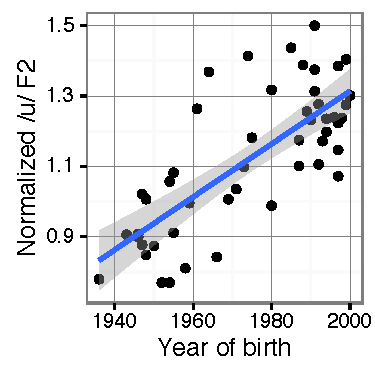
\includegraphics[scale=0.7]{uw_yob_small.pdf}
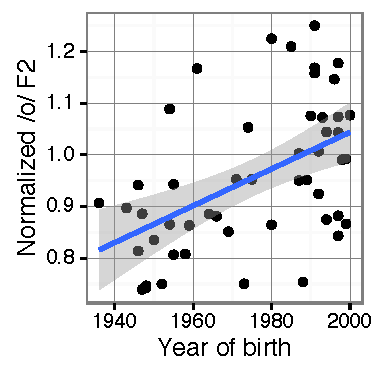
\includegraphics[scale=0.7]{ow_yob_small.pdf}
\caption{Apparent-time evidence of /u/ and /o/ fronting}
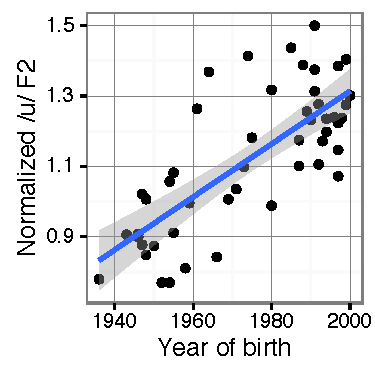
\includegraphics[scale=0.7]{uw_yob_small.pdf}
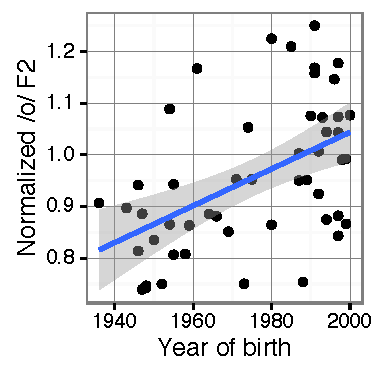
\includegraphics[scale=0.7]{ow_yob_small.pdf}
\caption{Apparent-time evidence of /u/ and /o/ diphthongization}
\end{figure}
\subsection{Dynamic change in /o/}

While considering Euclidean distance in isolation provides no evidence for dynamic change in /o/, plotting Euclidean distance and F2 values in two-dimensional space demonstrate how the sound change involves both fronting and diphthongization. Figure 3 demonstrates this.  The colored hulls show the output of a density-based clustering algorithm on these data, which identifies three groups of speakers -- those with back /o/ realizations and middle/high Euclidean distances; those with back /o/ realizations and low Euclidean distances, and those with fronted /o/ realizations and high Euclidean distances. It should also be noted that membership of each cluster is predictive of the age of the speaker --  back, diphthongal speakers are most likely to be in the oldest age group; back, monophthongal speakers are most likely to be in the middle or youngest age group, and speakers who produce front diphthongs are most likely to be in the youngest age group. The pattern appears to involve a reduction of the range of variation in diphthongization of back /o/ variants, and the adoption of very fronted, diphthongal variants among a subgroup of younger speakers. 

\begin{figure}[H]
\centering
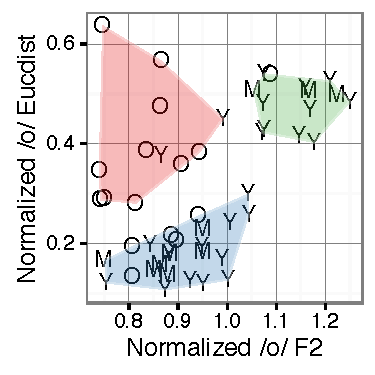
\includegraphics[scale=0.7]{ow_front_dip_small.pdf}
\end{figure}

In summary, the production data provide evidence for the fronting of /u/ and /o/ in this community. While /u/ fronting appears to proceed in a relatively uniform manner, /o/ fronting is appears to have taken place more slowly and spread less uniformly across the population. Considering the role of /o/ diphthongization in this process reveals that /o/ fronting is restricted to speakers with diphthongal /o/ -- while the fronting of monophthongal /o/ is in principle possible, and even attested in other Northern British varieties of English (reference), there appears to be an absence of fronted, monophthongal speakers in this sample, evident in the lack of datapoints in the bottom right-hand quadrant of figure x.

A schematization of the trajectory of change in /u/ and /o/ is provided below. The oldest speakers in the sample produce relatively back /u/ and /o/ variants, and exhibit variation in terms of /o/ diphthongization (i). The apparent conditional relationship between /u/ and /o/ fronting implies that change in /u/ actuated before that in /o/, allowing an intermediate state to be posited (ii). At this stage, the centralization of /u/ had begun, but /o/ remained relatively back. The present stage of the change (iii) involves further fronting of /u/, and the sharp separation of speakers into two groups with regard to their /o/ production -- those with very front diphthongs, and those with comparatively back monophthongs. 


\begin{table}[H]
\centering
\setlength{\tabcolsep}{0.5cm}
\label{haddican-results}
\begin{tabular}{llllllllll}
&i.&ii.&iii.&\\
/o/ &    o $\sim$ \textipa{oU} &  o $\sim$ \textipa{oU}        &  o       &  \textipa{\textschwa y}                                  && \\
/u/ &  \textipa{u} &  \textipa{0} &  \textipa{y} & \textipa{y}                    &           &                  &\\
&   &   &  &                    &           &                  &\\
\end{tabular}
\end{table}

This account of /u/ and /o/ fronting in York is generally consistent with Haddican et al.`s (2013) recent findings, with the exception of the presence of back \textipa{/o/} diphthongs among older speakers, which are absent from the Haddican et al. (2013) data. The patterning of these changes raises two key questions:

\begin{enumerate}[i)]
\item{What causes /u/ to front so rapidly and uniformly in comparison to /o/?}
\item{Why do younger speakers avoid fronting monophthongal /o/?}
\end{enumerate}

While a number of social, cognitive and linguistic factors might be invoked to explain these patterns, the remainder of this paper will focus on the proposal of Haddican et al. (2013), whose explanation centers around the social indexicality of variation in the changing vowels. The aim of this analysis is to demonstrate how a sociolinguistic account of language change can be empirically tested, by forming testable hypotheses regarding the relationship between listeners' social-indexical perception of changing forms and their production patterns. The following section will outline Haddican et al.`s (2013) proposal, use it to form a set of hypotheses regarding the social perception of /o/ and /u/, and evaluate those hypotheses using the social perception data.

\section{The social perception of \textipa{/u/} and \textipa{/o/} variation}

\subsubsection{Predictions based on Haddican et al. (2013)}

In order to explain differences in York speakers adoption of /u/ and /o/ fronting, Haddican et al. (2013) present a detailed argument regarding the social-indexical significance of variation in the two vowels. With regard to the relative uniformity of change in /u/ vis-a-vis /o/, the authors propose that the fronting of /u/ is less important as a social-indexical resource to York speakers in comparison to the fronting and diphthongization of /o/. Under this account, this relative lack of social indexing allows /u/ fronting to propagate rapidly and relatively uniformly across the community, since the adoption of fronted /u/ variants will have limited social consequence for speakers. In contrast, /o/ diphthongization is claimed to be strongly associated with socioeconomic status and `local' regional identity. Such claims are reasonable, since the diphthongization of the mid vowels is known to be a shibboleth of Northern/Southern English identity, at least in production (refs...). The implication of Haddican et al.`s (2013) proposal is that change in /o/ might be slower and less uniform than change in /u/ due to the participation of /o/ in a pattern of social indexing. 

The author's third key claim is that fronted, monophthongal /o/ is associated with a stigmatized working-class stereotype, the `chav'. This stereotype, reflecting an individual who is typically unemployed and engages in antisocial behaviour, has become a key feature of popular discourses around social class in the United Kingdom (see e.g. Hayward \& Yar, 2006). Haddican et al. (2013) provide convincing evidence from ethnographic interviews that this social category is important to younger York residents, and propose that the absence of fronted, monophthongal /o/ in their data may be explained by younger speakers' avoidance of forms enregistered as `chav' speech. 

Haddican et al.`s (2013) social-indexical account of variation and change in /o/ and /u/ represents a common pattern of argument in sociolinguistic work -- inferring a social signalling system based on observed production patterns. One way of thinking about their proposal is to express it as a set of hypotheses regarding social categories represented in multidimensional space (here expressed simply as Euclidean distance and F2). These social categories may include `macro-level' meanings such as \textsc{local} or \textsc{working class}, or more locally-specific personae such as \textsc{chav}. This is visualized below:

\begin{figure}[H]
\centering


\includegraphics[scale=0.25]{u_hypothesis_space.png}
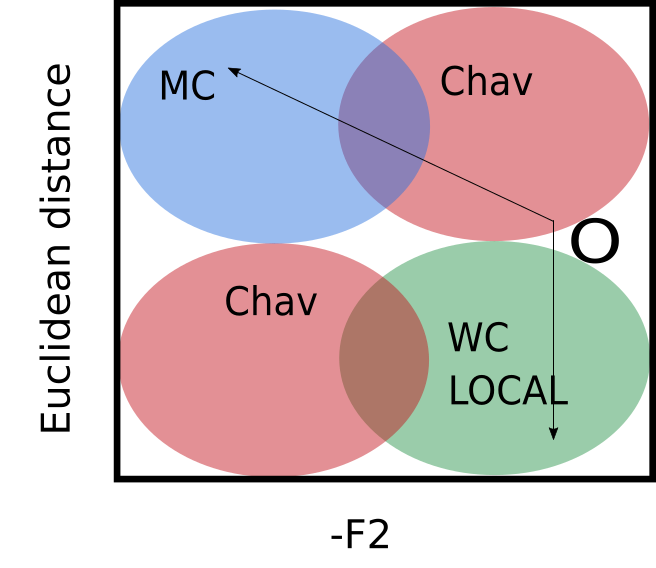
\includegraphics[scale=0.25]{o_hypothesis_space.png}
\end{figure}

Figure x includes an addition to the argument presented in Haddican et al. (2013), with the inclusion of the hypothesis that back /o/ monophthongs are also enregistered as part of the \textsc{chav} persona. Since back /o/ diphthongs as well as fronted /o/ monophthongs are absent from the speech of younger speakers, it is reasonable to extend Haddican et al.`s (2013) proposal to include these forms. 

The perception data allow the explicit testing of these hypotheses -- by analysing the way listeners assign variation in the changing forms to the social categories presented in the experiment, it is possible to verify the general pattern proposed above, as well as to explore the consistency with which individuals can identify the proposed social meanings. This is achieved through framing the hypotheses as statements about probabilities, then estimating those probabilities through a statistical model. Specifically:

\begin{enumerate}[(a)]
\item{The probability of a \textsc{working-class} selection should be higher for monophthongal /o/ variants than diphthongal /o/ variants}
\item{The probability of a \textsc{local} selection should be higher for monophthongal /o/ variants than diphthongal /o/ variants}
\item{Variation in /u/ should have a comparatively smaller effect on the probability of a \textsc{working-class} or \textsc{local} selection compared to variation in /o/}
\item{The probability of a \textsc{chav} selection should be higher for fronted, monophthongal /o/ than back, monophthongal /o/}
\item{The probability of a \textsc{chav} selection should be higher for back, diphthongal /o/ than front, diphthongal /o/}
\item{(d) and (e) will interact with listener year of birth, with younger listeners showing a larger effect}
\end{enumerate}

\subsection{Model selection}

These probabilities were estimated using multilevel logistic regression fit for each vowel on each social dimension. The analyses presented here focus on models for the \textsc{working class} dimension (all \textsc{working class} vs all \textsc{middle class} images), the \textsc{rural} dimension (all \textsc{rural} vs all \textsc{non-rural} images), and the \textsc{chav} category (the \textsc{chav} image vs all others).  Baseline models predicted the selection of the social category modeled with random intercepts, by-listener random slopes for \textit{variant}, and random slopes for sound sample within \textit{variant}.
The relative fit of these models was compared with more complex ones, including terms for the variant heard, the listener's year of birth, their score on the mobility index, and the interactions of those factors.
\newpage
\begin{figure}[!htpb]
\caption{AIC for each candidate model, ordered by complexity}
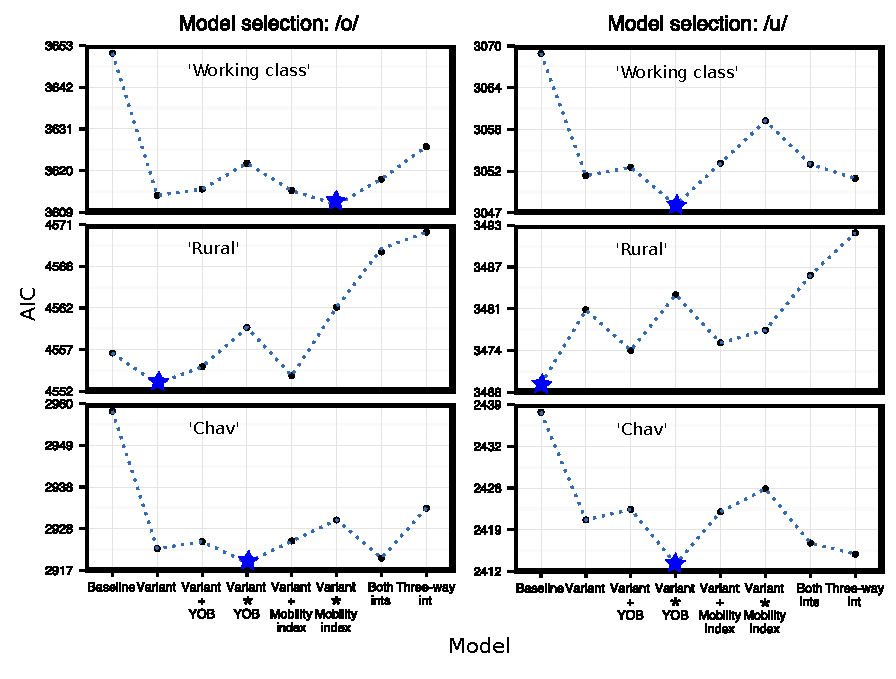
\includegraphics[scale=0.9]{model_comparison.pdf}
\end{figure}
\vspace{-.65cm}

 The relative fit of these models is visualized in figure x.x, which plots the Akaike Information Criterion value for each model specification, arranged in order of model complexity. A lower AIC value indicates a better fit to the data.The best-fitting models are marked with a star. In terms of social class selections, the models for both /u/ and /o/ include the \textit{variant} term, confirming that listeners were able to use variation in these vowels as a reliable cue to socioeconomic status and to the \textsc{chav} subcategory. \textsc{rural}selections were reliably affected by variation in /o/, but not /u/. The best models for \textsc{working class} also include interaction terms for listener mobility (/o/) and year of birth (/u/), and the best models for \textsc{chav} include interaction terms for year of birth, indicating that listeners of different ages and social backgrounds behaved differently in the social perception task. Overall, it can be seen that, where included in the final model, the variant term contributes much more than the interaction terms to overall fit. For example, the `Working class' and `Chav' models for /o/ with lowest AIC include interaction terms, but the addition of these terms appears to improve fit only marginally. In order to test the reliability of these effects, a parametric bootstrap of likelihood ratio tests was conducted, in each case comparing the lowest-AIC model with the next best candidate. 

\subsection{Results: Main effects}
\subsubsection{\textsc{working class} selections}
\begin{figure}[H]
\centering
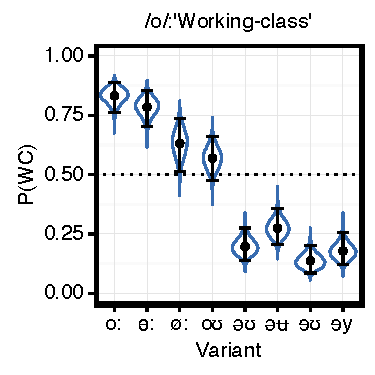
\includegraphics[scale=0.8]{ow_class.pdf}
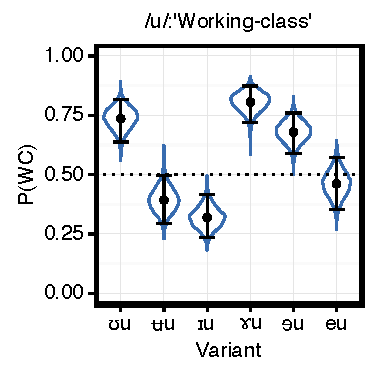
\includegraphics[scale=0.8]{uw_class.pdf}
\end{figure}
Figure x demonstrates how variation in /u/ and /o/ effected listeners' responses in on the social class dimension. The points represent the mean predicted probability of a \textsc{working class} selection, with error bars showing the upper and lower bounds of the Highest Posterior Density interval, estimated through 10000 samples. For /o/, there is a clear effect of diphthongization, with more diphthongal variants reliably cueing the selection of a middle class image, and monophthongal variants cueing the selection of working-class image. The only exception to this pattern is back, diphthongal /o/; the fact that the HPD interval for this variant crosses zero means that we cannot be certain that it had a reliable effect in either direction, but the fact that the interval is biased above the p=.5 line suggests that listeners tended to select working-class images when hearing this variant. Monophthongs all reliably predict the selection of a working-class image, but the strength of this effect weakens for more fronted variants. In summary, we observe a robust effect of diphthongization, with diphthongs predicting middle-class selections, and a smaller effect of fronting whereby more fronted variants cue middle-class selections. Note that this effect holds for both diphthongs and monophthongs, in contrast to what might be predicted based on Haddican et al. (2013). 

In terms of responses to /u/, there is a clear effect of fronting whereby fronter /u/ variants are more likely to cue middle-class selections and back variants are more likely to cue working-class selections. /u/ diphthongization seems to be weakly associated with \textsc{working class}, in that diphthongization weakens the effect of fronting (evident in the shallower slope of fronting across more diphthongal /u/ variants, and in the fact that the HPD interval for fronted, diphthongal /u/ crosses the p=.5 line. These effects are very suprising given the predictions formed earlier, where it was suggested that /u/ fronting would have a limited effect on listeners' social selections than /o/ diphthongization. 
\subsubsection{\textsc{rural} selections}
\begin{figure}[H]
\centering
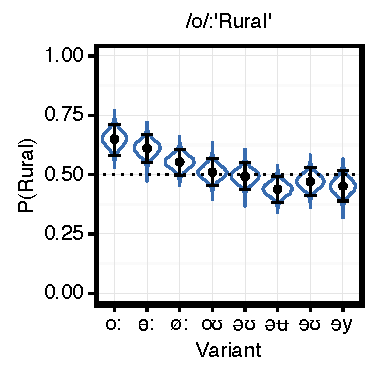
\includegraphics[scale=0.8]{ow_local.pdf}
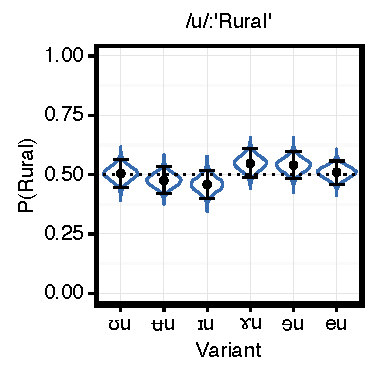
\includegraphics[scale=0.8]{uw_local.pdf}
\end{figure}
In terms of selections on the urban-rural dimension, only the model for /o/ was significantly improved by the inclusion of the \textit{variant} term, but predictions from comparable models for both vowels are provided here for comparison. /u/ variants show no reliable effect on listeners' urban/rural selections, while /o/ shows a weak but reliable effect for monophthongal variants. While diphthongs all show no reliable effect (in that the HPD interval crosses p=.5), monophthongs reliably cue the selection of a rural charachter. The fact that only monophthongs show reliable effects suggests that while /o/ monophthongs are associated with rural speech, the converse is not true of diphthongs. Overall, the results are broadly consistent with our earlier predictions -- /u/ shows no evidence of being associated with rural identity, while /o/ monophthongs show a reliable association with this social category.
\subsubsection{\textsc{chav} selections}
\begin{figure}[H]
\centering
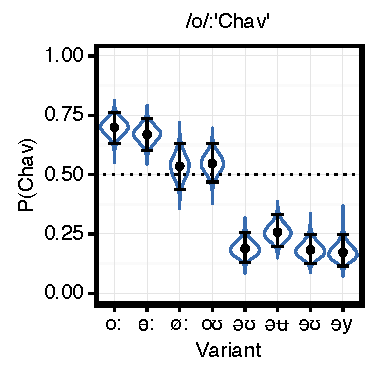
\includegraphics[scale=0.8]{ow_chav.pdf}
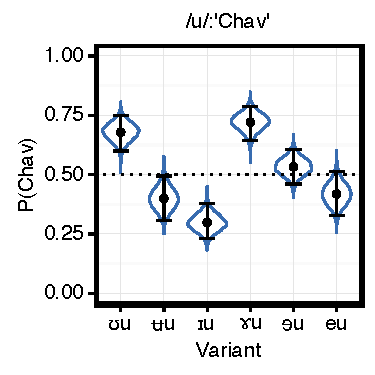
\includegraphics[scale=0.8]{uw_chav.pdf}
A key prediction based on Haddican et al.'s (2013) proposal was that fronted /o/ monophthongs would be associated with the 'Chav' subcategory. Figure x plots predictions for 'Chav' images vs all other, conditional on the variant of /o/ and /u/ heard. It is clear that these results provide no support for this proposal -- rather, they mirror the effects for general  \textsc{working class} selections. While the most back /o/ variants reliably cue \textsc{chav} selections, fronted /o/ shows no reliable effect, and the overall trend is for fronting to \textit{lower} the probablity of a \textsc{chav} selection. Similarly to the \textsc{working class} selections, more back /u/ variants increase the probablity of a \textsc{chav} selection, and this effect is weakly mediated by diphthongization. Once again, these results contrast strongly with the Haddican et al. (2013) proposal -- /u/ shows robust social perception effects where none were predicted, and the effect of fronting appears to run in the opposite direction to what would be expected under the Haddican et al. (2013) account.
\end{figure}
\subsection{Results: Listener variation}
A further prediction made in section x was that listeners would vary in their social perception of variation in /o/ and /u/. In particular, it was predicted that the 'Chav' association between fronted /o/ monophthongs and back /o/ diphthongs would be strongest among younger listeners. While no evidence was found for the predicted relationship between /o/ variation and \textsc{chav}, the data still provide evidence of variation in social perception, demonstrated below.
\subsubsection{\textsc{working class} selections}
\begin{figure}[H]
\centering
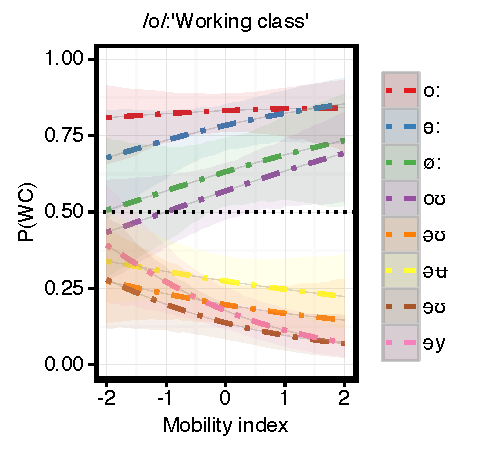
\includegraphics[scale=0.8]{ow_class_dim3.pdf}
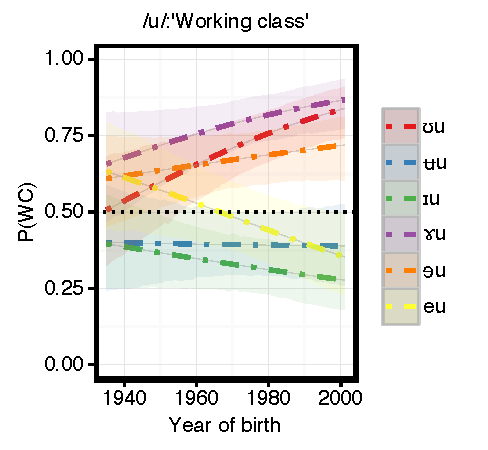
\includegraphics[scale=0.8]{uw_class_age.pdf}
\end{figure}
Figure x demonstrates variation in social class selections. For /o/, there is a significant effect of listener mobility, with more mobile listeners generally more sensitive to the monophthong-diphthong distinction as a cue to socioeconomic status. The largest variation appears to be in the perception of the most fronted diphthong and most back monophthong -- these variants have a limited effect on the responses of less mobile listeners, suggesting that those listeners hear them as comparatively unmarked. In contrast, more mobile listeners tend to associated these variants with middle-class characters.

/u/ selections show now evidence of variation in terms of mobility, but a significant effect of listener age, shown in figure x. Older listeners are generally less sensitive to fronting as a cue to socioeconomic status.
\subsubsection{\textsc{chav} selections}
\begin{figure}[H]
\centering
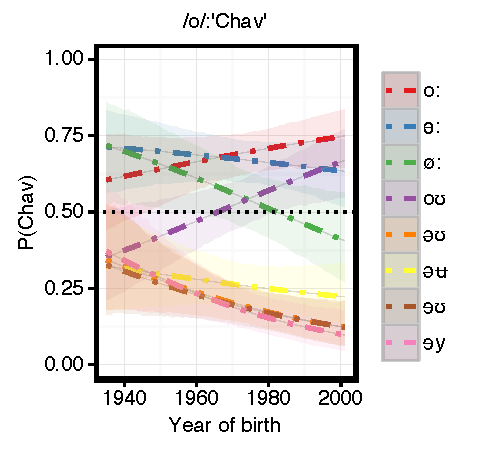
\includegraphics[scale=0.8]{ow_chav_age.pdf}
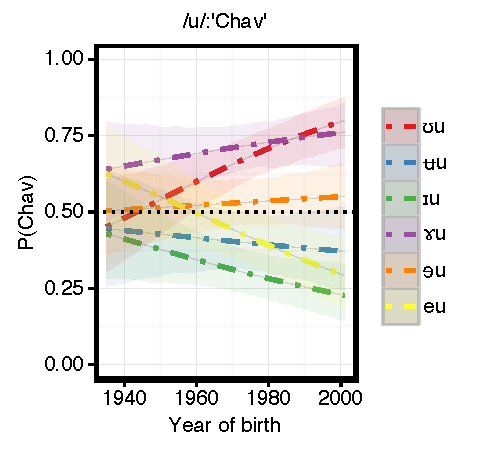
\includegraphics[scale=0.8]{uw_chav_age.pdf}
\end{figure}
\section{Conclusion}
\section{References}
\bibliographystyle{pwpl.bst}
\nocite{*}
\bibliography{reviewbib_short.bib}
\end{document}
